\section{\strace{} in Aktion}

\subsection{Analyse eines einfachen Programms}

\begin{frame}[t,fragile]
  \frametitle{Beispielhafte Analyse eines Python-Programms}

  \begin{lstlisting}
% strace notfound.py > output.txt
  \end{lstlisting}

  \centering
  \begin{columns}
    \column{\dimexpr\paperwidth}
    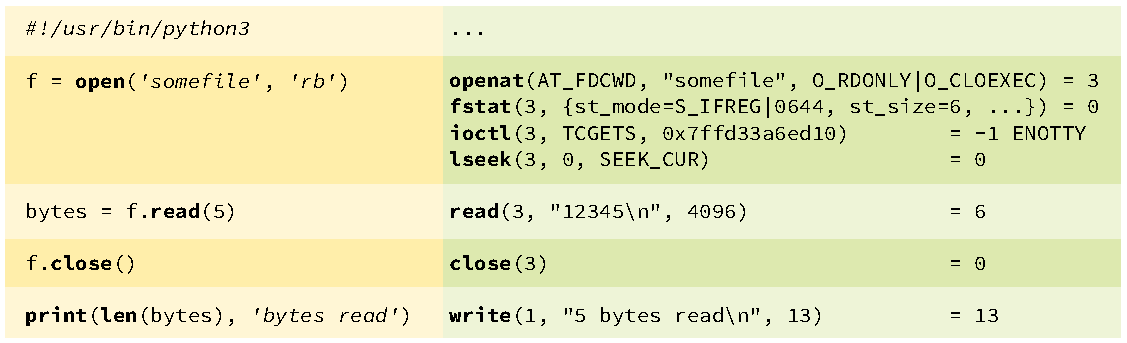
\includegraphics[width=\paperwidth]{../images/sample-listing.pdf}
  \end{columns}

\end{frame}

\begin{frame}[t,fragile]
  \frametitle{Fehlerfall}

  \begin{lstlisting}
% rm somefile 
% strace notfound.py > output.txt
  \end{lstlisting}

  \begin{exampleblock}{\vspace*{-2ex}}
  \begin{lstlisting}
...
openat(AT_FDCWD, "somefile", O_RDONLY|O_CLOEXEC) = 
   -1 ENOENT (Datei oder Verzeichnis nicht gefunden)
...
  \end{lstlisting}
  \end{exampleblock}


\end{frame}

\subsection{Kindprozesse und Threads}

\begin{frame}
  \frametitle{Protokollierung in einer Datei}

  

\end{frame}

\subsection{Protokollierung in einer Datei}

\subsection{\strace{} einschränken}


\subsection{Strings}
